\section{Desarrollo del \textit{frontend}}
\label{dev:sec:desarrollo_frontend}

Definida la base de datos y desarrollado el \textit{backend}, el \textit{frontend} es la última parte de la plataforma que resta por ser definido y desarrollado. El \textit{frontend} es con lo que el usuario interactúa directamente, y es la responsable de mostrar la información para que este pueda realizar las acciones que desee.

Existen múltiples tecnologías que permiten desarrollar el \textit{frontend} de una plataforma web, pero en este caso se ha optado por utilizar React, un \textit{framework} de JavaScript que hoy en día es uno de los más utilizados para el desarrollo de aplicaciones web. Precisamente del hecho de que React sea un estándar de facto en el desarrollo web, se deriva la decisión de haber utilizado esta tecnología. Es un \textit{framework} muy potente, respaldado por una gran cantidad de documentación, recursos y de una enorme empresa como es Meta (anteriormente conocida como Facebook), la cual es su creadora y mantenedora. Esto asegura que React se mantenga actualizado y sea compatible con las últimas tecnologías web.

A pesar de que React funciona con JavaScript, siguiendo lo mencionado en la sección \ref{mt:subsec:frontend}, se ha optado por utilizar TypeScript. TypeScript es un superconjunto de JavaScript que añade tipado estático y otras características que facilitan el desarrollo y mantenimiento del código. Esto permite detectar errores en tiempo de compilación, lo que mejora la calidad del código y reduce la probabilidad de errores en tiempo de ejecución. Estos aspectos son especialmente importantes en un proyecto de gran envergadura, donde la complejidad del código puede aumentar rápidamente. Como se pretende que la plataforma siga evolucionando y creciendo, el uso de TypeScript facilita la escalabilidad del proyecto y evita problemas a largo plazo.

Con estos puntos claros, se ha procedido a desarrollar el \textit{frontend} de la plataforma. Este proceso se ha dividido en principalmente dos fases: la estructuración del proyecto y el desarrollo de las diferentes vistas y componentes que componen la plataforma.

\subsection{Estructuración del proyecto}
\label{dev:subsec:estructuracion_proyecto}

Las estructuras de los proyectos desarrollados con React pueden variar dependiendo de las necesidades del proyecto y de las preferencias del equipo de desarrollo. Sin embargo, existen algunas convenciones y buenas prácticas que se suelen seguir para mantener el código organizado y fácil de mantener.

En este caso, se ha optado por una estructura que se divide en principalmente cuatro carpetas principales:

\begin{itemize}
    \item \texttt{src/components}: Esta carpeta reúne todos los componentes reutilizables de la aplicación. En React, los componentes son las unidades básicas que conforman la interfaz: pueden ir desde elementos sencillos como botones hasta estructuras más complejas como formularios completos. Para mantener una buena organización, se divide esta carpeta en subcarpetas: una para los componentes comunes (usados en múltiples partes de la aplicación) y otras para los componentes específicos de cada funcionalidad o sección.
    \item \texttt{src/routes}: En esta carpeta se encuentran definidas todas las rutas de la aplicación utilizando la librería @tanstack/react-router. La estructura de rutas sigue una organización jerárquica que refleja la navegación de la aplicación, permitiendo agrupar rutas relacionadas en subcarpetas. Cada archivo de ruta incluye tanto la definición del componente que debe renderizarse como los datos que necesita cargar.
    \item \texttt{src/services}: Esta carpeta contiene los servicios encargados de realizar las peticiones HTTP al \textit{backend} utilizando la librería axios. Cada servicio agrupa las funciones relacionadas con un recurso concreto de la aplicación (por ejemplo, pedidos o productos), lo que permite centralizar la lógica de comunicación con el servidor.
    \item \texttt{src/types}: Esta carpeta contiene tanto las definiciones de tipos TypeScript como los esquemas de validación de la aplicación. Los tipos se utilizan para garantizar una correcta tipificación del código en toda la aplicación, mejorando la seguridad y legibilidad. Por su parte, los esquemas, definidos con la librería zod, se emplean para validar los datos introducidos por el usuario antes de enviarlos al servidor, asegurando que cumplan con las reglas establecidas (por ejemplo, formatos, campos obligatorios o rangos de valores).
\end{itemize}

Esta estructura queda plasmada en la figura \ref{fig:dev:estructura_archivos}, donde se puede observar la estructura de carpetas que almacenan todo el código del \textit{frontend}. En la siguiente sección se detallará el desarrollo de las vistas y los componentes que componen cada una de ellas, lo que permitirá una mejor comprensión de la figura.

\begin{figure}[H]
    \centering
    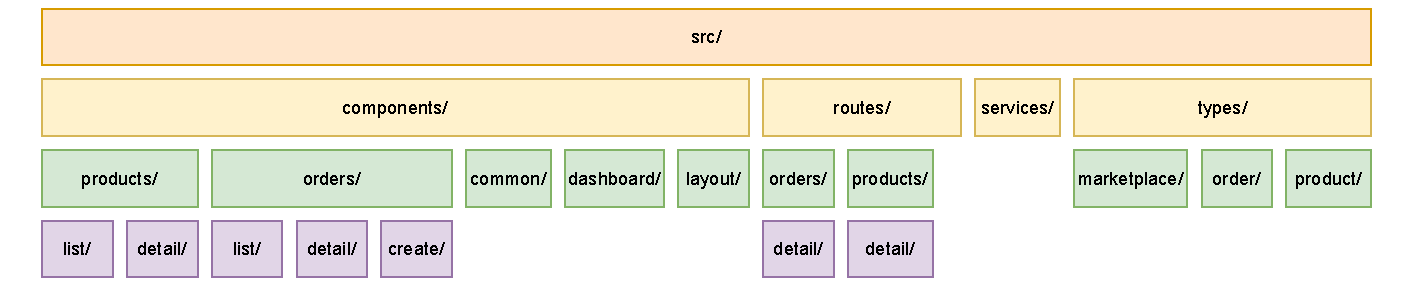
\includegraphics[width=0.95\textwidth]{figures/design_develop/estructura_archivos.pdf}
    \caption{Estructura de archivos del \textit{frontend} de la plataforma.}
    \label{fig:dev:estructura_archivos}
\end{figure}

\subsection{Desarrollo de vistas y componentes}
\label{dev:subsec:desarrollo_vistas_componentes}

Las vistas constituyen la interfaz de usuario de la plataforma. Son el conjunto de elementos con los que el usuario interactúa directamente y, en términos coloquiales, representan la cara visible de la aplicación. Por este motivo, el desarrollo de vistas implica también el desarrollo de componentes, ya que cada vista se construye a partir de múltiples componentes que se combinan para ofrecer una visualización coherente y funcional de la aplicación.

Antes de comenzar con el desarrollo de las vistas, es fundamental tener claro cómo deben ser accesibles las distintas funcionalidades de la plataforma para el usuario final. Por este motivo, resulta útil remitir a la sección \ref{dev:subsec:bloques_funcionalidades}, donde se definieron los bloques funcionales principales. A modo de resumen, las funcionalidades clave que debe ofrecer la plataforma son las siguientes:

\begin{itemize}
    \item \textbf{Gestión de pedidos}:
          \begin{itemize}
              \item Centralización de los pedidos procedentes de los distintos canales de venta.
              \item Creación manual de nuevos pedidos.
              \item Edición de pedidos existentes.
          \end{itemize}
    \item \textbf{Gestión de productos}:
          \begin{itemize}
              \item Centralización de los productos provenientes de los distintos canales de venta.
              \item Asignación de productos a canales de venta específicos.
              \item Edición de los atributos de los productos en cada canal de venta.
          \end{itemize}
\end{itemize}

El desarrollo de estas funcionalidades debe enfocarse en ofrecer una experiencia de usuario ágil e intuitiva, permitiendo una gestión eficiente de los canales de venta. El objetivo es que la plataforma se convierta en una herramienta imprescindible para la administración diaria de los distintos \textit{marketplaces} y que el usuario no pierda tiempo en tareas repetitivas o tediosas.

Es importante señalar que los usuarios de la plataforma no disponen de permisos para crear ni editar canales de venta. La incorporación de un nuevo canal es una tarea gestionada exclusivamente por la plataforma, ya que implica un análisis previo, así como la implementación y configuración de la \gls{api} correspondiente, entre otros aspectos técnicos. El usuario final puede asignar productos a los canales ya disponibles, pero no tiene control sobre su creación o configuración.

Teniendo en cuenta las funcionalidades definidas, la plataforma debe contar con dos vistas principales: una para la gestión de pedidos y otra para la gestión de productos. Como añadido a estas vistas, se ha incluido una vista de inicio que proporciona una visión general de la plataforma y permite observar datos generales del estado de los pedidos y productos.

Así pues, para centralizar las tres vistas principales se ha creado un menú lateral de navegación que permite al usuario acceder fácilmente a cada una de ellas, tal como se muestra en la figura \ref{fig:dev:ss:menu_lateral}. Este menú está presente en todas las vistas de la plataforma, permitiendo que el usuario pueda acceder a cada una de las secciones principales de forma rápida. De momento el menú cuenta con tres secciones: \textit{Dashboard}, \textit{Orders} y \textit{Products}. Sin embargo, está diseñado para que, en el futuro, se puedan añadir nuevas secciones fácilmente así permitiendo la expansión de nuevas funcionalidades.

\begin{figure}[H]
    \centering
    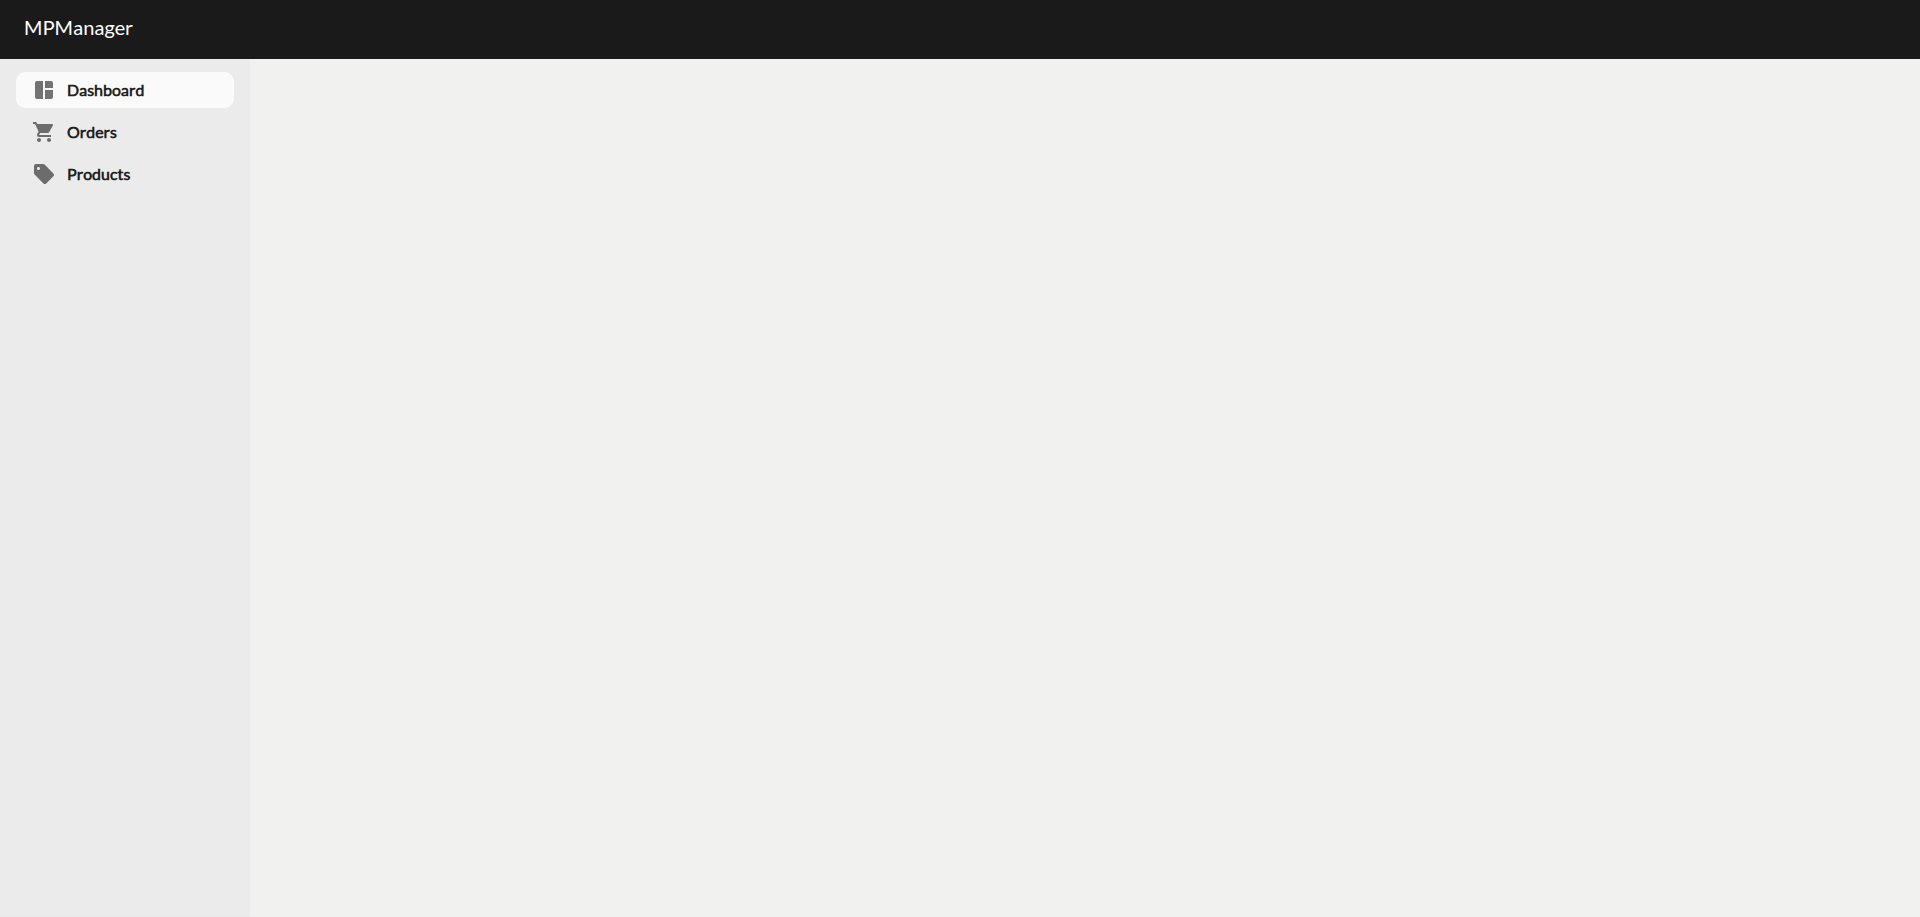
\includegraphics[width=0.8\textwidth]{figures/design_develop/screenshots/menu_lateral.png}
    \caption{Menú lateral de navegación de la plataforma.}
    \label{fig:dev:ss:menu_lateral}
\end{figure}

El orden de las secciones del menú lateral sigue una lógica que facilita la navegación. En primer lugar, se encuentra la sección \textit{Dashboard}, que proporciona una visión general del estado de la plataforma, permitiendo al usuario obtener información rápida sobre los pedidos y productos. A continuación, se sitúa la sección \textit{Orders}, que permite gestionar los pedidos de forma centralizada. Finalmente, la sección \textit{Products}, donde se pueden gestionar los productos disponibles en los distintos canales de venta.

No obstante, el orden de desarrollo de las vistas no ha seguido este mismo orden, sino que se ha desarrollado primero la vista de pedidos, seguida de la vista de productos y, por último, la vista de inicio. El orden entre las vistas de pedidos y productos no es relevante, ya que ambas son bastante independientes una de la otra. Sin embargo, la vista de inicio se ha desarrollado al final para poder incluir en ella información relevante sobre el estado de los pedidos y productos, que se obtiene de las vistas anteriores. Por este mismo motivo, a continuación se detallará el desarrollo de las vistas según el orden con el que se han implementado, pues es seguramente el orden más lógico para comprender como todo funciona e interactúa.

\subsubsection{Vista de pedidos}
\label{dev:subsubsec:vista_pedidos}

La vista de pedidos es una de las más importantes de la plataforma, ya que permite gestionar todos los pedidos provenientes de los distintos canales de venta. Gestionar los pedidos implica poder verlos, editarlos y crear de nuevos. Así pues, dicha vista se ha dividido en tres:

\begin{itemize}
    \item \textbf{Vista general de pedidos}: Esta vista permite al usuario ver todos los pedidos que ha recibido la plataforma, independientemente del canal de venta del que provengan. Se pueden filtrar los pedidos por el canal de ventas además de poder buscarlos por su identificador o el nombre del cliente.
    \item \textbf{Vista detallada de pedido}: Esta vista permite al usuario ver un pedido concreto, así como editarlo. Se pueden ver todos los detalles del pedido, incluyendo los productos que lo componen, el estado del pedido y la información del cliente. Además, se pueden realizar acciones como editar el estado del pedido o añadir nuevos productos al mismo.
    \item \textbf{Vista de creación de pedido}: Esta vista permite al usuario crear un nuevo pedido. Se pueden seleccionar los productos que componen el pedido, así como introducir la información del cliente y el canal de venta al que pertenece el pedido.
\end{itemize}

\begin{figure}[H]
    \centering
    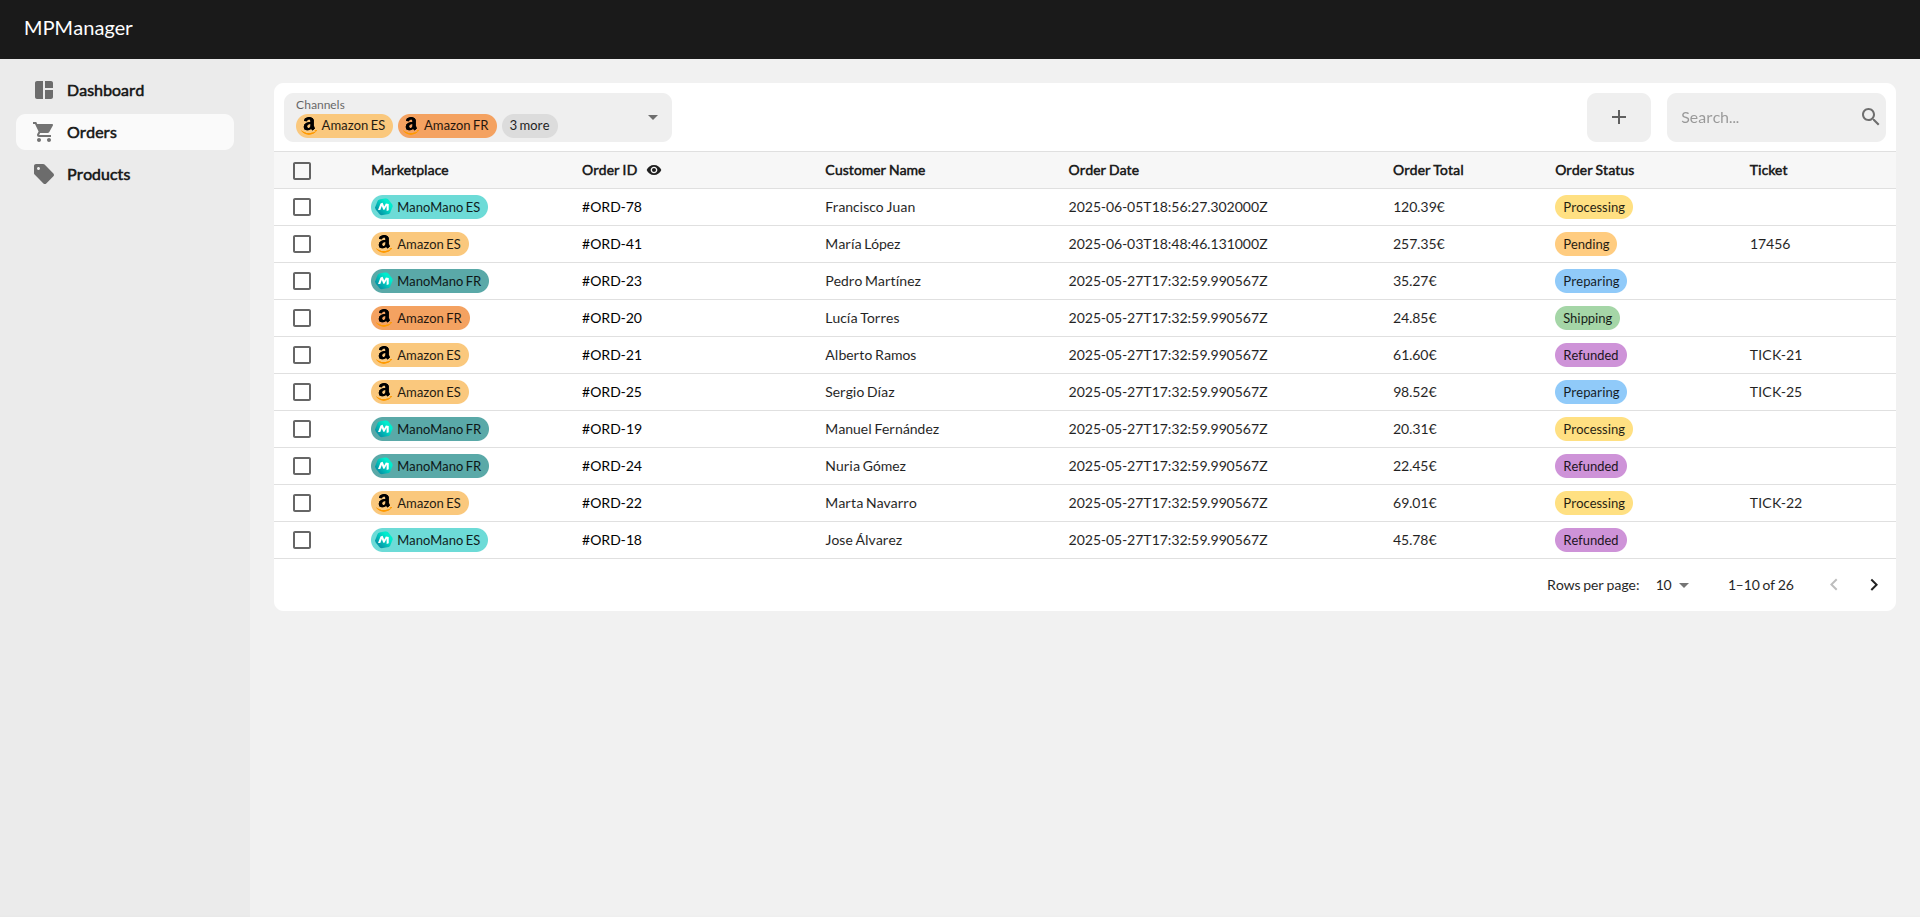
\includegraphics[width=0.8\textwidth]{figures/design_develop/screenshots/tabla_pedidos.png}
    \caption{Vista general de pedidos con algunos pedidos de ejemplo.}
    \label{fig:dev:ss:vista_general_pedidos}
\end{figure}

La primera de las vistas, la vista general de pedidos, es la que se muestra en la figura \ref{fig:dev:ss:vista_general_pedidos}. Esta vista está principalmente compuesta por una tabla que muestra los pedidos recibidos, mostrando el canal de venta del que provienen, el identificador del pedido, el nombre del cliente, la fecha de creación del pedido, el importe total y el estado del mismo. Adicionalmente, se ha añadido un campo de búsqueda que permite filtrar los pedidos por el identificador del pedido o el nombre del cliente; y un filtro por canal de venta que permite ver únicamente los pedidos de los canales seleccionados.

Sin embargo, se puede observar que la tabla no muestra todos los pedidos de la plataforma, sino que muestra únicamente los 10 últimos pedidos recibidos. Como un usuario puede tener cientos o miles de pedidos, es necesario implementar una paginación que permita navegar entre los distintos pedidos. Esta paginación implementada es la discutida en la sección \ref{dev:subsubsec:paginacion_endpoints}, y permite al usuario cambiar entre las distintas páginas de pedidos, seleccionar cuántos pedidos se quieren ver por página (10, 25, 50 o 100), buscar pedidos concretos y filtrar por canal de venta. De esta forma, para cada cambio de página, de búsqueda o de filtro, se realiza una petición al \textit{backend} para obtener los pedidos correspondientes a la página, búsqueda o filtros seleccionados.

Para cargar todo el contenido de la vista, se hacen dos peticiones al \textit{backend}: una para obtener los pedidos y otra para obtener los canales de venta disponibles. Por otro lado, todos los componentes que componen la vista estan en la carpeta \texttt{src/components/orders/orders-list} y son llamados desde el archivo \texttt{src/routes/orders/index.tsx}, que es el encargado de definir la ruta.

\begin{figure}[H]
    \centering
    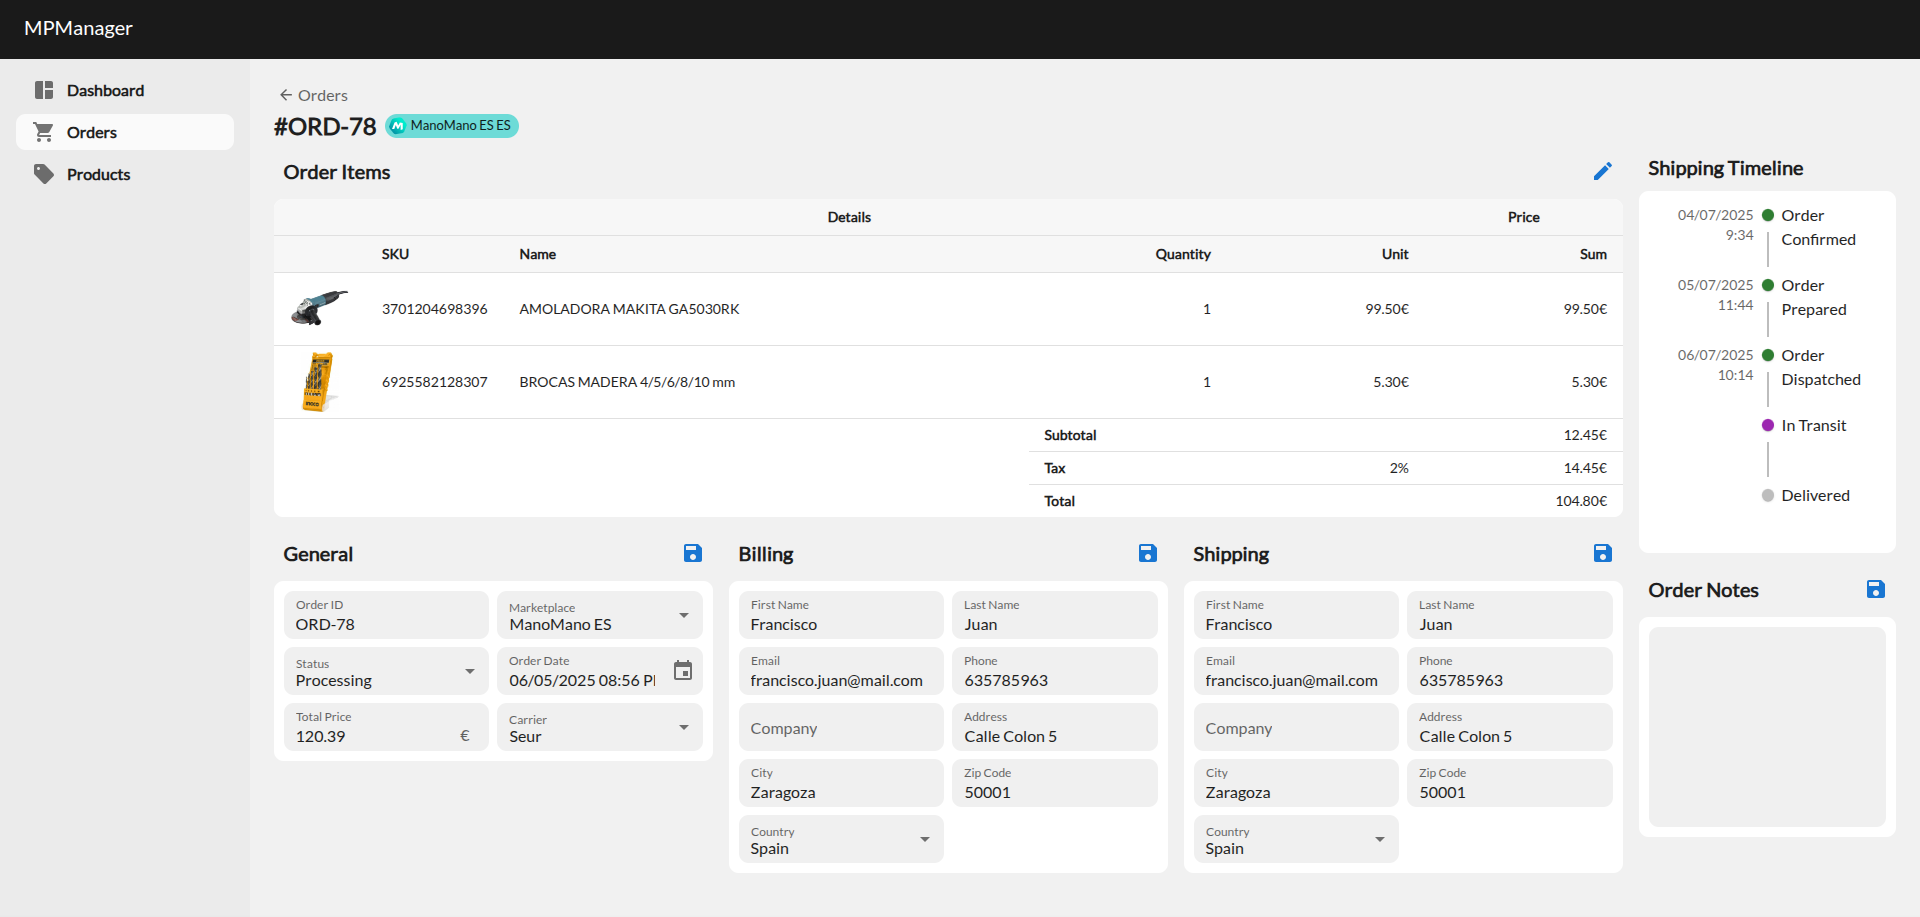
\includegraphics[width=0.8\textwidth]{figures/design_develop/screenshots/detalle_pedidos.png}
    \caption{Vista detallada de un pedido concreto.}
    \label{fig:dev:ss:vista_detallada_pedidos}
\end{figure}

Pulsando sobre un pedido concreto de la tabla, se accede a su vista detallada, que se muestra en la figura \ref{fig:dev:ss:vista_detallada_pedidos}. En esta vista se pueden ver todos los detalles del pedido, incluyendo los artículos que lo componen, la información general del pedido y la información del cliente. Adicionalmente, se puede revisar cómo ha ido evolucionando el estado del pedido a lo largo del tiempo, ya que se muestra un historial de cambios de estado del pedido, y se pueden añadir notas para registrar información adicional relevante.

Existe la posibilidad también de editar el pedido, tanto los productos que lo componen como la información general y del cliente. Sin embargo, existe una restricción importante: solo se pueden editar los pedidos que hayan sido creados manualmente por el usuario. Los pedidos que provienen de los canales de venta no pueden ser editados, ya que su información es gestionada directamente por el canal. Esto asegura la integridad de los datos y evita posibles inconsistencias en la información.

Tal como se muestra en la figura \ref{fig:dev:ss:campos_editables_pedido}, los únicos campos que se pueden editar en los pedidos provenientes de los canales de venta son los siguientes:

\begin{itemize}
    \item \textbf{Estado del pedido:} El usuario puede cambiar el estado del pedido a uno de los estados disponibles en el desplegable. Esto es útil para indicar que el pedido ha sido preparado, enviado o entregado, entre otros.
    \item \textbf{Transportista}: El usuario puede seleccionar el transportista que se debe encargar de enviar el pedido. Esto es útil para llevar un control de los envíos y poder realizar un seguimiento del pedido.
    \item \textbf{Notas del pedido:} El usuario puede añadir notas al pedido para registrar información adicional relevante. Estas notas pueden ser útiles para el seguimiento del pedido o para registrar información adicional que no se encuentra en los campos del pedido.
    \item \textbf{Dirección de facturación y envío:} El usuario tiene la posibilidad de editar la dirección de facturación y de envío asociadas al pedido. Esta funcionalidad resulta especialmente útil, ya que dichos datos son utilizados por la \gls{api} del transportista para calcular el coste del envío y generar la etiqueta correspondiente. Sin embargo, si el formato de la dirección no es correcto, la \gls{api} puede devolver un error, lo que impediría completar el envío del pedido.
\end{itemize}

\begin{figure}[H]
    \centering
    \begin{subfigure}{\linewidth}
        \centering
        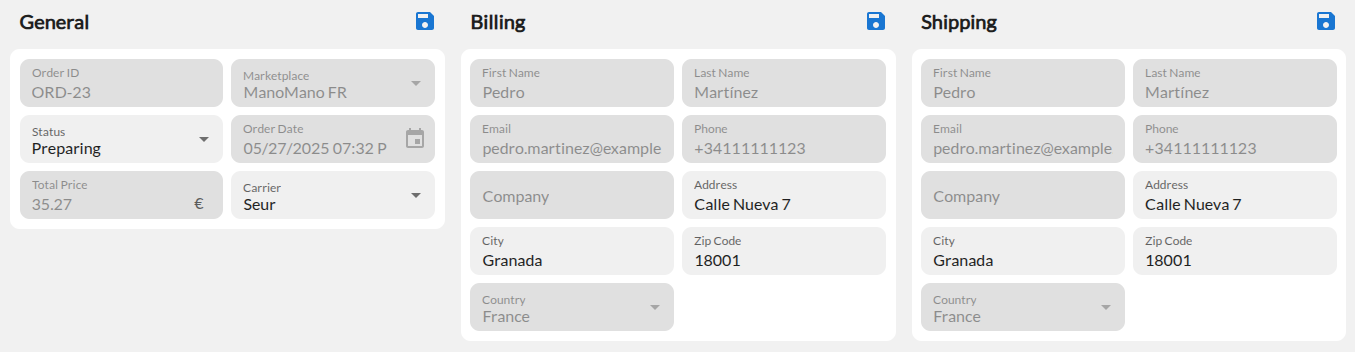
\includegraphics[width=0.8\linewidth]{figures/design_develop/screenshots/campos_bloqueados.png}
        \caption{Campos de un pedido creado automáticamente por el canal de venta.}
    \end{subfigure}
    \par\vspace{0.6cm}
    \begin{subfigure}{\linewidth}
        \centering
        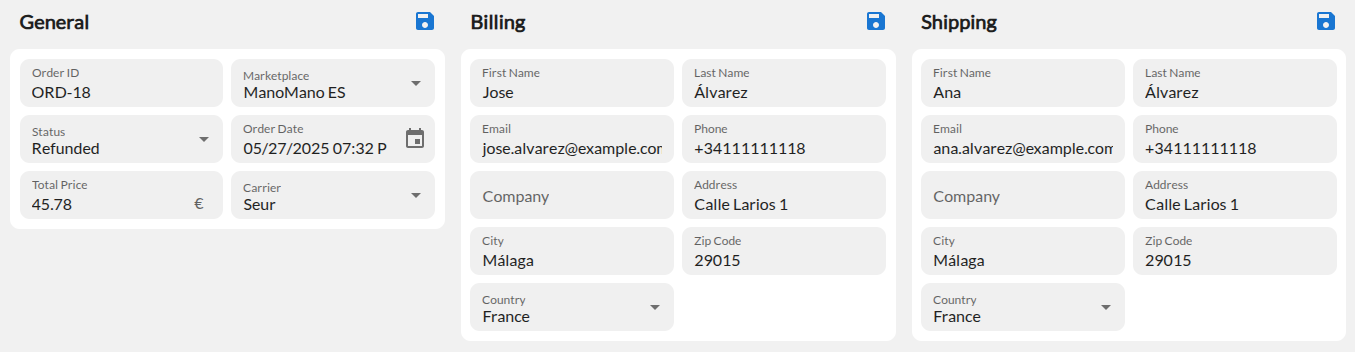
\includegraphics[width=0.8\linewidth]{figures/design_develop/screenshots/campos_no_bloqueados.png}
        \caption{Campos de un pedido creado manualmente por el usuario.}
    \end{subfigure}
    \par\vspace{0.3cm}
    \caption{Campos editables de un pedido dependiendo de su origen.}
    \label{fig:dev:ss:campos_editables_pedido}
\end{figure}

Por otro lado, en pedidos creados manualmente, se pueden añadir o quitar artículos al pedido, así como editar los ya existentes. Para realizar estas acciones se debe pulsar el icono de edición que se encuentra en la parte superior derecha de la tabla de productos. Esto abrirá el modal que se muestra en la figura \ref{fig:dev:ss:modal_edicion_productos_pedido}. Cabe señalar que un modal es una ventana emergente que se superpone a la vista actual y permite al usuario realizar acciones sin abandonar la vista en la que se encuentra. Es normalmente un recurso muy útil para realizar acciones rápidas o para mostrar información adicional sin necesidad de cambiar de vista, de manera que se adapta a la perfección a esta situación.

\begin{figure}[H]
    \centering
    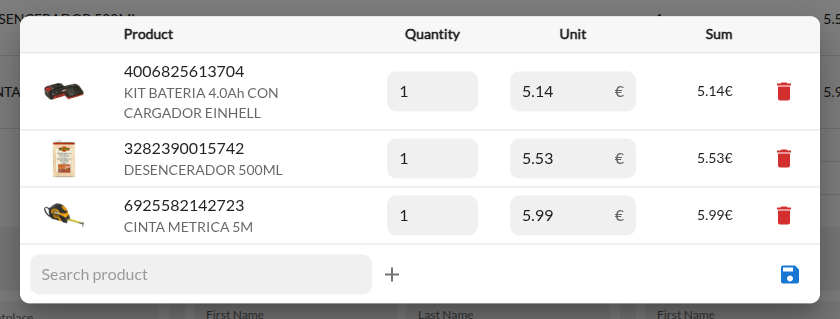
\includegraphics[width=0.7\textwidth]{figures/design_develop/screenshots/modal_edicion_productos_pedido.png}
    \caption{Modal de edición de productos de un pedido.}
    \label{fig:dev:ss:modal_edicion_productos_pedido}
\end{figure}

Este modal incluye características bastante complejas, como es la búsqueda de productos dinámicamente. A medida que el usuario escribe en el campo de búsqueda el nombre o \gls{sku} del producto, se realiza una petición al \textit{backend} para obtener los productos que coincidan con la información introducida. Solo los productos que se encuentran en el canal de venta del pedido se mostrarán en la lista de resultados, lo que asegura que solo se puedan añadir productos válidos al pedido. Además, para evitar que se hagan demasiadas peticiones al \textit{backend}, se ha implementado un \textit{debounce} de 500 milisegundos, lo que significa que la búsqueda solo se realizará si el usuario deja de escribir durante ese tiempo, funcionalidad que se puede ver en la figura \ref{fig:dev:ss:busqueda_debounced}. Esto reduce la carga en el servidor y mejora la experiencia del usuario al evitar peticiones innecesarias.

\begin{figure}[H]
    \centering
    \begin{subfigure}{0.45\linewidth}
        \centering
        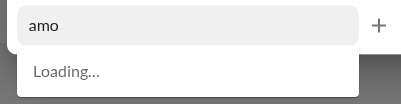
\includegraphics[width=\linewidth]{figures/design_develop/screenshots/busqueda_debounced_loading.png}
        \caption{Desplegable de búsqueda de productos con el \textit{debounce} mientras espera la respuesta del \textit{backend}.}
    \end{subfigure}
    \hfill
    \begin{subfigure}{0.45\linewidth}
        \centering
        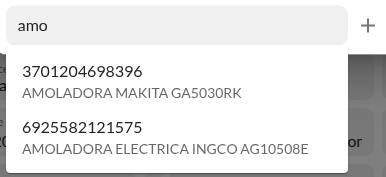
\includegraphics[width=\linewidth]{figures/design_develop/screenshots/busqueda_debounced.png}
        \caption{Desplegable de búsqueda de productos con los resultados obtenidos de la respuesta del \textit{backend}.}
    \end{subfigure}
    \par\vspace{0.3cm}
    \caption{Proceso de búsqueda de productos con \textit{debounce}.}
    \label{fig:dev:ss:busqueda_debounced}
\end{figure}

Cuando el usuario ha añadido, eliminado o editado los artículos del pedido, puede pulsar el icono de guardado para almacenar los cambios realizados. Esto enviará una petición al \textit{backend} con los nuevos productos y cantidades. Aquí es donde se hace uso de las características de acciones masivas explicadas en la sección \ref{dev:subsubsec:actualizacion_creacion_eliminacion_masiva}.

Finalmente, para cargar la vista detallada de un pedido se realizan dos peticiones al \textit{backend}: una para obtener el pedido concreto y otra para obtener los canales de venta disponibles. Todos los componentes que componen la vista se encuentran sitaudos en la carpeta \texttt{src/components/orders/detail} y son llamados desde \texttt{src/routes/orders/\$orderId.tsx}, que es el encargado de definir la ruta.

La última de las vistas de pedidos es la vista de creación manual de pedido. Para acceder a ella, el usuario debe estar en la vista de productos y pulsar el ícono "$+$", situado a la izquierda de la barra de búsqueda.

Crear un pedido manualmente es una tarea considerablemente tediosa, ya que hay que introducir una amplia variedad de datos. Por este motivo, se ha optado por dividir la creación del pedido en tres pasos:

\begin{enumerate}
    \item \textbf{Información general:} \\
          En el primer paso se debe introducir la información general del pedido, como el canal de venta al que pertenece, el identificador del pedido, la fecha de creación, el estado del pedido, entre otros. Parte de esta información, como es el ticket, es opcional y se puede dejar en blanco si no se dispone de ella. Otros de los campos, como el canal de venta o el método de pago, son obligatorios y deben ser seleccionados entre las opciones disponibles de su desplegable.
          \begin{figure}[H]
              \centering
              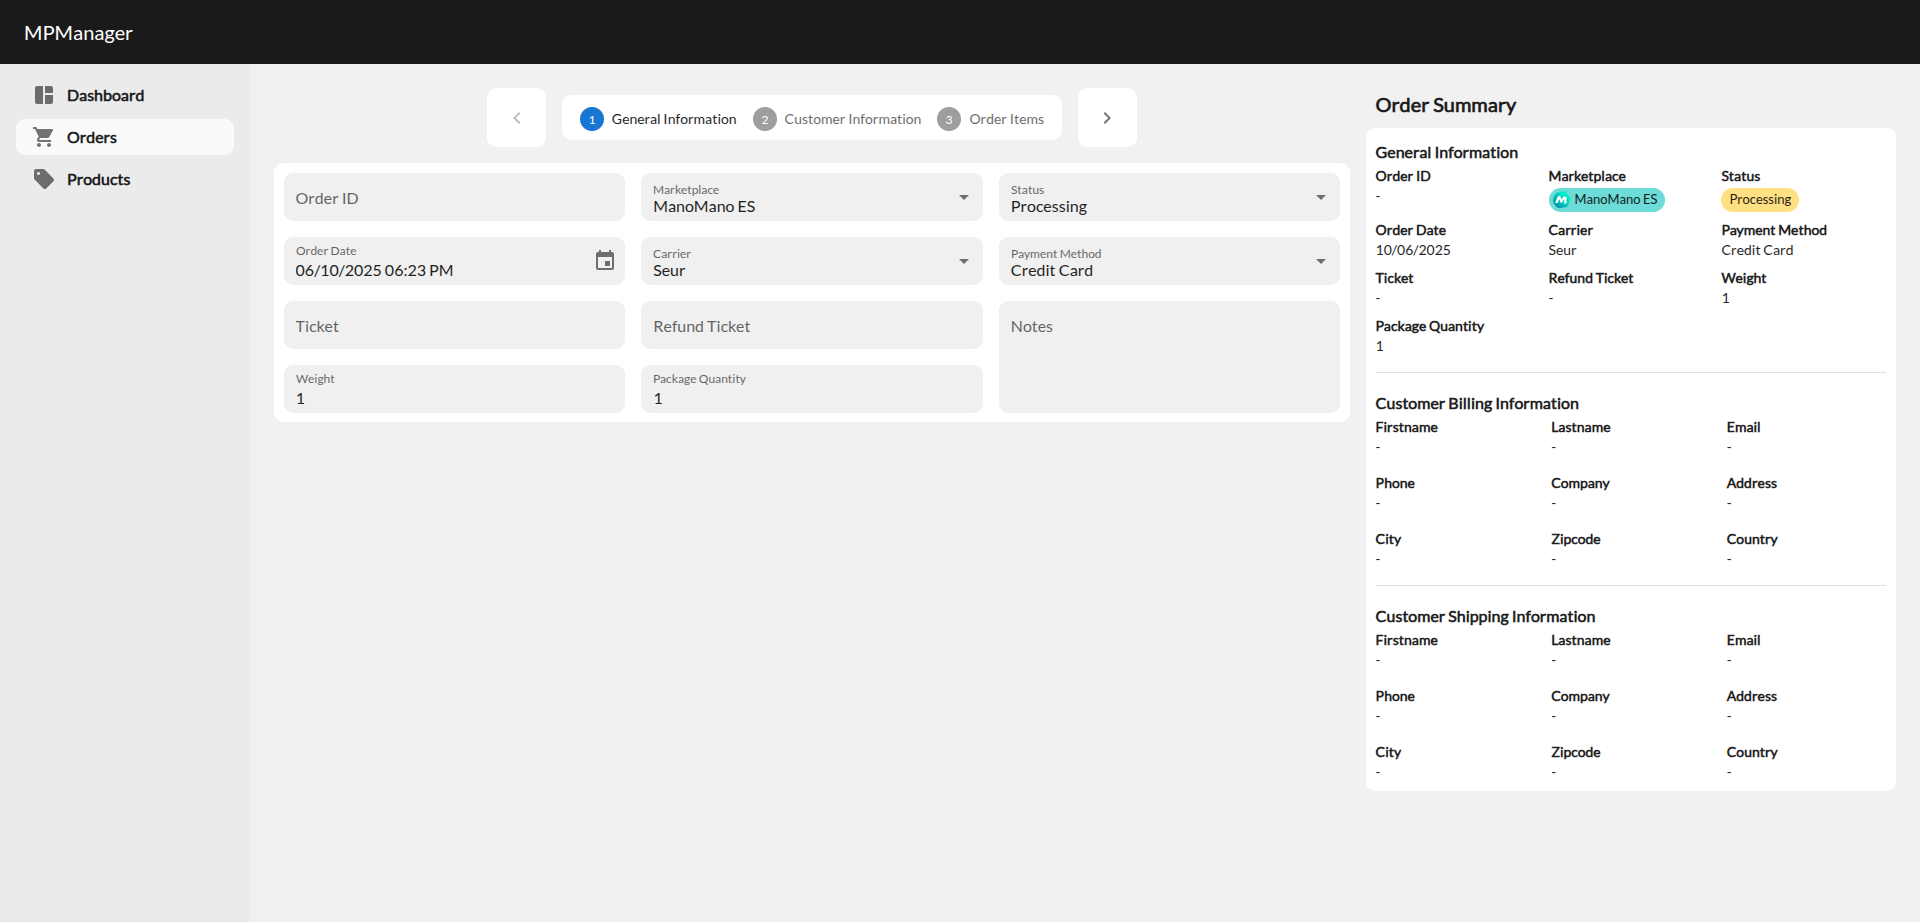
\includegraphics[width=0.8\textwidth]{figures/design_develop/screenshots/creacion_pedido_1.png}
              \caption{Información general del pedido.}
              \label{fig:dev:ss:creacion_pedido_1}
          \end{figure}
    \item \textbf{Información del cliente:} \\
          En el segundo paso se debe introducir la información del cliente, tanto la de facturación como la de envío. En este caso, todos los campos son obligatorios, ya que es necesario disponer de toda la información del cliente para poder gestionar el pedido correctamente. Sin embargo, para hacer el formulario más ágil existen dos posibles acciones que se pueden realizar:
          \begin{figure}[H]
              \centering
              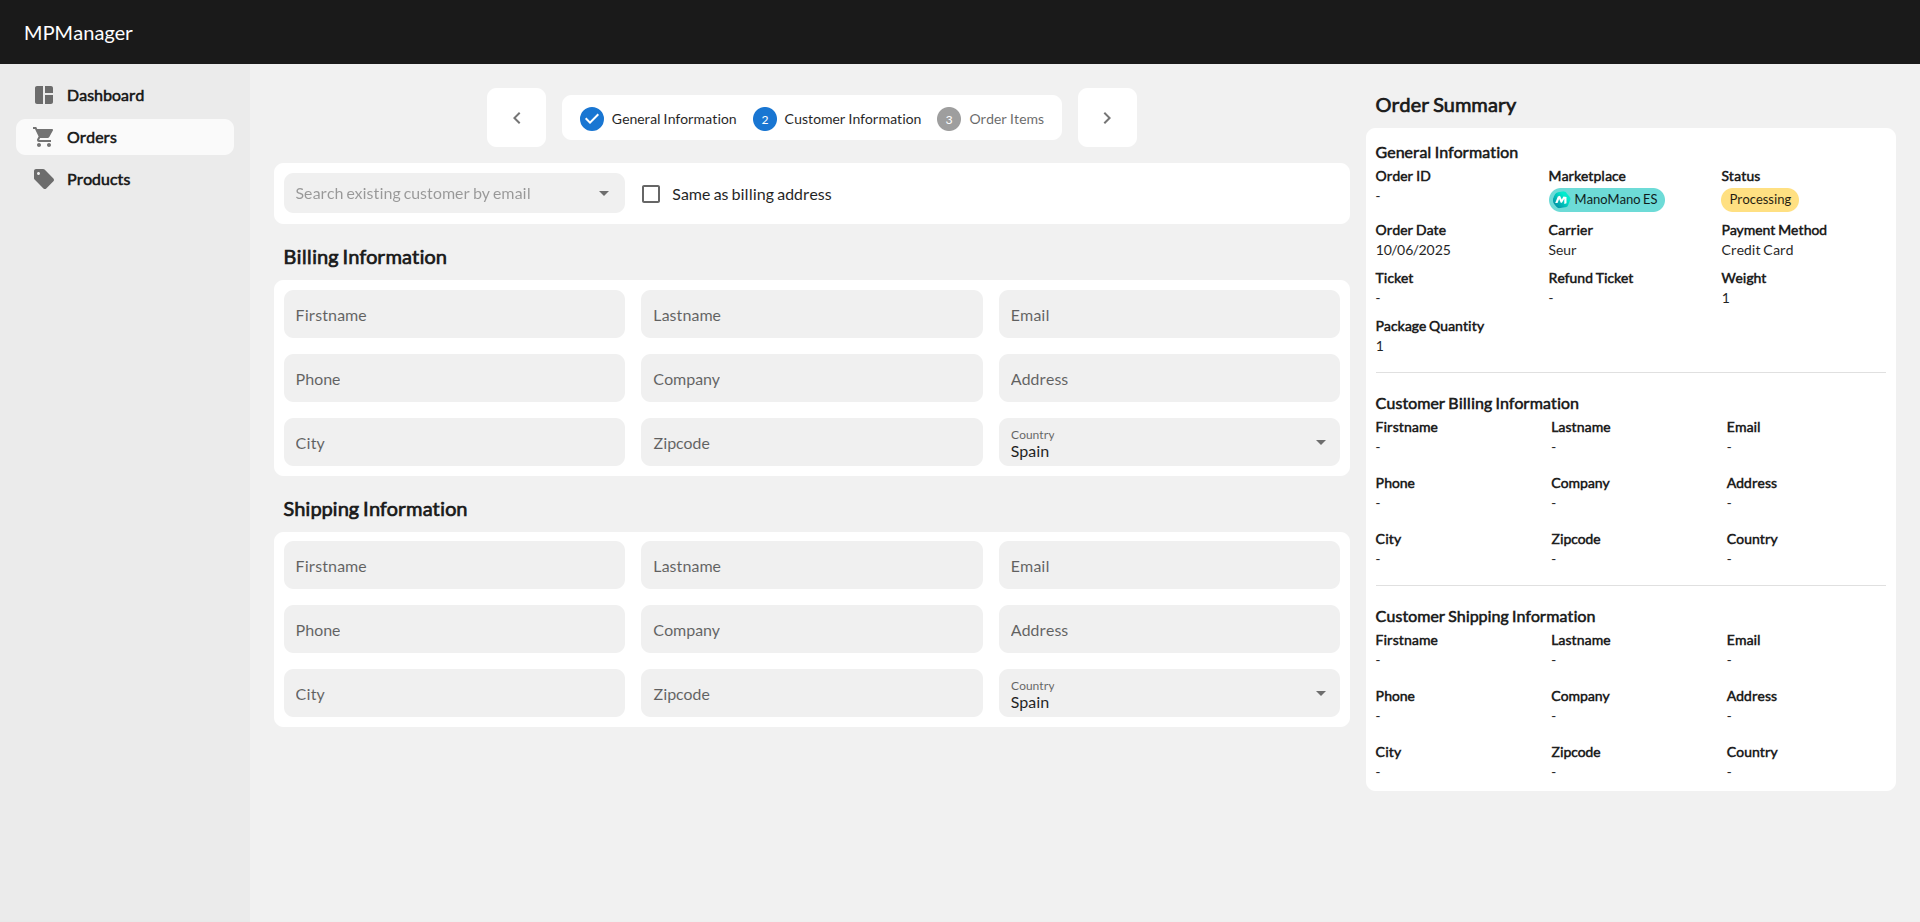
\includegraphics[width=0.8\textwidth]{figures/design_develop/screenshots/creacion_pedido_2.png}
              \caption{Información del cliente del pedido.}
              \label{fig:dev:ss:creacion_pedido_2}
          \end{figure}
          \begin{itemize}
              \item \textbf{Rellenar automáticamente los campos si el cliente ya existe:} Si el cliente ya existe en la base de datos, este puede ser buscado mediante su correo electrónico. El método de búsqueda funciona de forma similar al de la búsqueda de productos, es decir, mediante un \textit{debounce}. Si se encuentra un cliente con ese correo, los campos de información del cliente se rellenarán automáticamente con los datos del cliente encontrado y se bloquearán para evitar que se modifiquen.
              \item \textbf{Clonar los datos de facturación a los de envío:} Si el cliente tiene la misma información de facturación y envío, se puede marcar la opción de \textit{Same as billing} para clonar los datos de facturación a los de envío. Con esta opción marcada los campos de envío se rellenarán automáticamente con los datos de facturación a medida que se vayan introduciendo y se bloquearán para evitar que se modifiquen.
          \end{itemize}
          \begin{figure}[H]
              \centering
              \begin{subfigure}{0.45\linewidth}
                  \centering
                  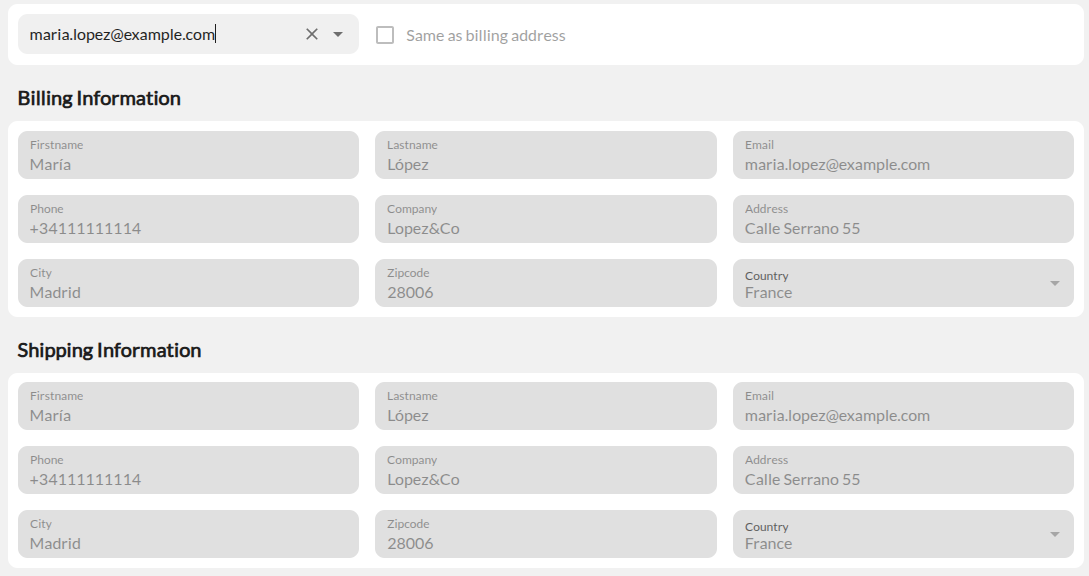
\includegraphics[width=\linewidth]{figures/design_develop/screenshots/creacion_pedido_2_bloqueado_search.png}
                  \caption{Campos de información del cliente bloqueados al buscar un cliente existente.}
              \end{subfigure}
              \hfill
              \begin{subfigure}{0.45\linewidth}
                  \centering
                  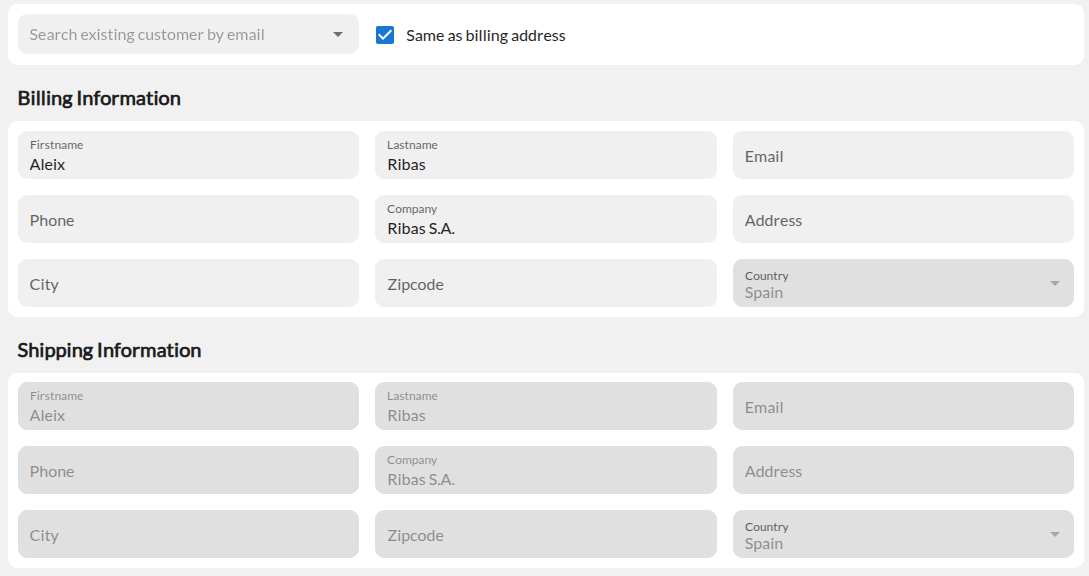
\includegraphics[width=\linewidth]{figures/design_develop/screenshots/creacion_pedido_2_bloqueado_check.png}
                  \caption{Campos de información del cliente bloqueados al clonar los datos de facturación.}
              \end{subfigure}
              \par\vspace{0.3cm}
              \caption{Campos de información del cliente bloqueados.}
              \label{fig:dev:ss:creacion_pedido_2_bloqueados}
          \end{figure}
    \item \textbf{Información de productos:} \\
          Por último, en el tercer paso se deben añadir los artículos que componen el pedido. Para ello, se puede buscar un producto concreto mediante su nombre o \gls{sku}, y añadirlo al pedido con la cantidad y el precio correspondientes. Al igual que en la vista detallada de pedidos y en la búsqueda de clientes, en la búsqueda de productos también se ha implementado un \textit{debounce} para evitar hacer demasiadas peticiones al \textit{backend} y una mejor experiencia de usuario. El precio total del pedido se calcula automáticamente en función de los productos añadidos y sus cantidades, además de que el impuesto aplicable se calcula automáticamente en función del canal de venta seleccionado.
          \begin{figure}[H]
              \centering
              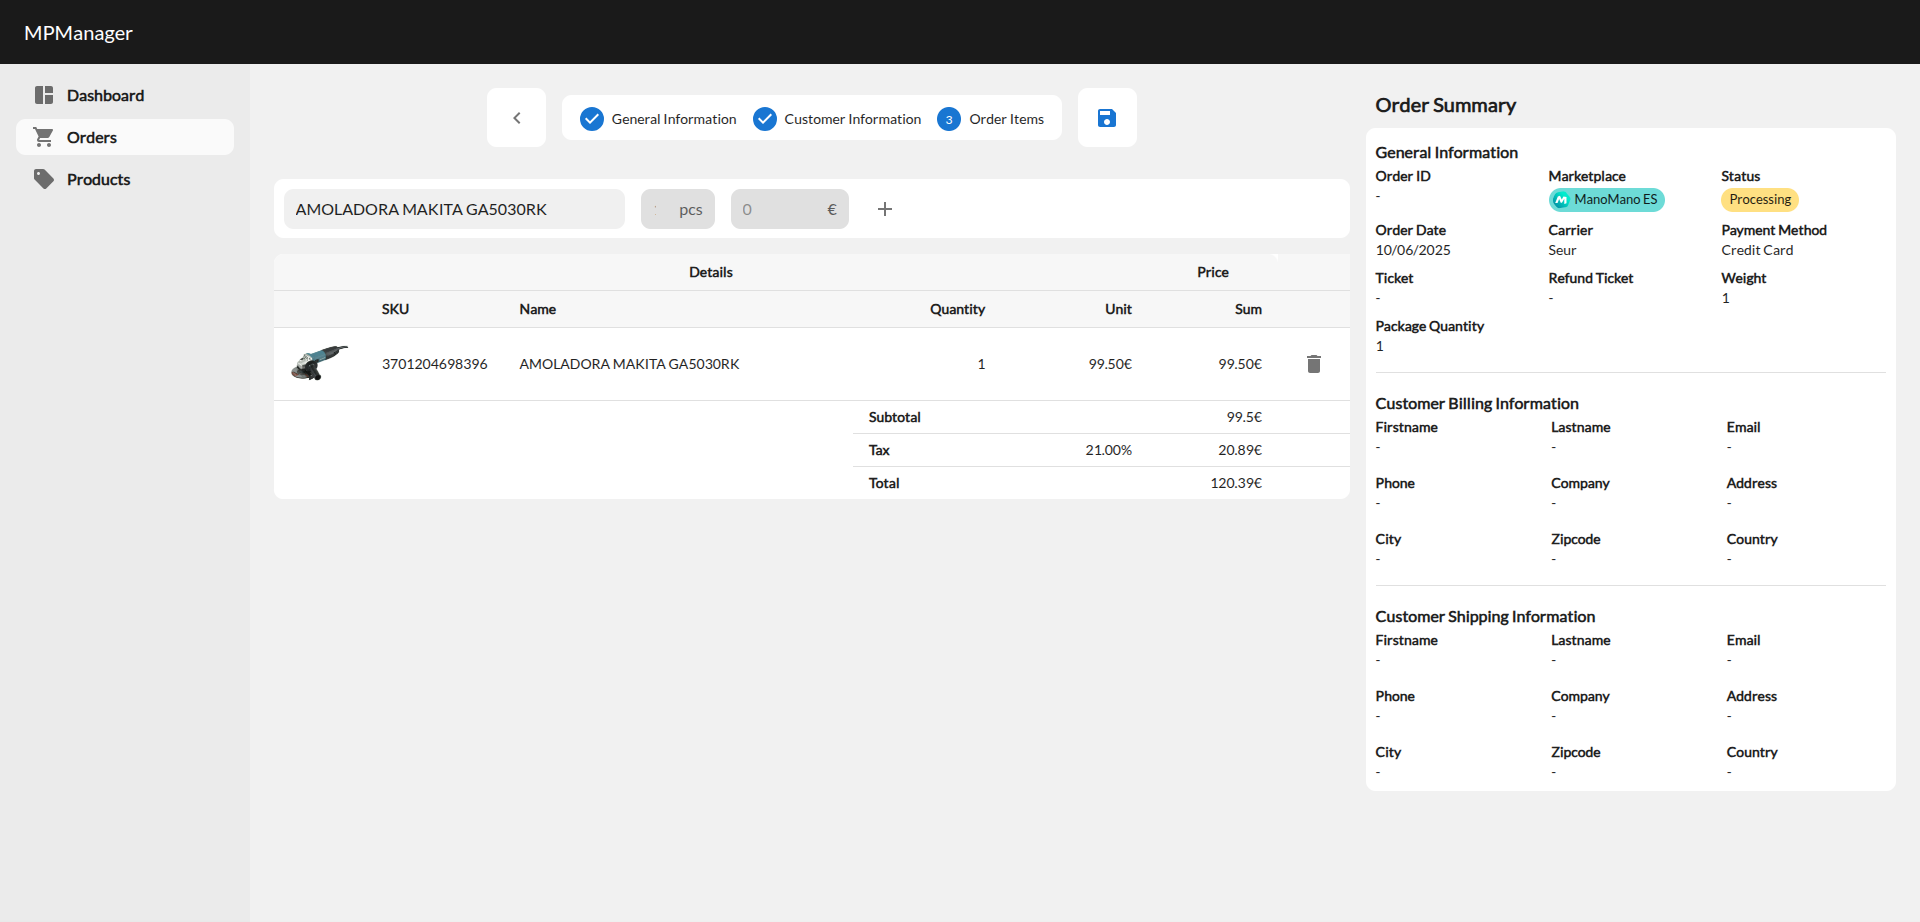
\includegraphics[width=0.8\textwidth]{figures/design_develop/screenshots/creacion_pedido_3.png}
              \caption{Información de productos del pedido.}
              \label{fig:dev:ss:creacion_pedido_3}
          \end{figure}
\end{enumerate}

Como se puede observar a lo largo de las distintas figuras, para cambiar entre los distintos pasos se ha implementado una barra de navegación que permite al usuario ir hacia adelante y hacia atrás entre los pasos.

Para finalizar la creación del pedido, el usuario debe pulsar el icono de guardar que se encuentra en dicha barra de navegación cuando ha completado todos los pasos. Esto enviará una petición al \textit{backend} para crear el nuevo pedido con la información introducida. Si todo es correcto, el pedido se añadirá a la lista de pedidos y estará disponible para su gestión.

Sin embargo, en la vista de creación de pedidos hay otro elemento que aún no ha sido mencionado: la tarjeta lateral de resumen del pedido. Esta tarjeta se encuentra en la parte derecha de la vista y muestra un resumen de la información introducida en los distintos pasos. A medida que el usuario va completando los pasos, la tarjeta se actualiza automáticamente para reflejar la información introducida. Esto permite al usuario tener una visión general del pedido que está creando y asegurarse de que toda la información es correcta antes de guardarlo. No obstante, esta tarjeta tiene otra utilidad adicional, la cual justifica su presencia: indica al usuario que campos son incorrectos cuando se intenta guardar el pedido.

Si algún campo es incorrecto o no se ha completado, la tarjeta mostrará un error en dicho campo y, pasando el ratón por encima, se mostrará un mensaje indicando qué es lo que falta por completar o qué es lo que está mal. Este comportamiento se puede observar en la figura \ref{fig:dev:ss:tarjeta_resumen_pedido}, donde se muestra un ejemplo de cómo se indica al usuario que el número de pedido es obligatorio y debe ser introducido para poder guardar el pedido.

\begin{figure}[H]
    \centering
    \begin{subfigure}{0.45\linewidth}
        \centering
        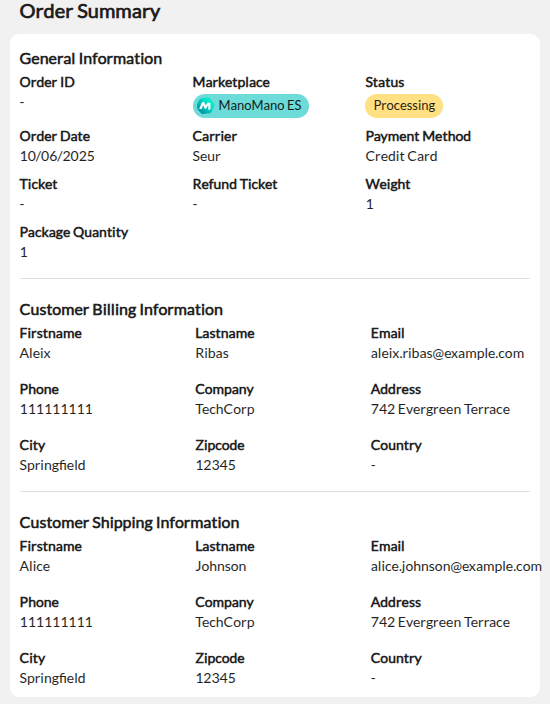
\includegraphics[width=\linewidth]{figures/design_develop/screenshots/tarjeta_resumen_antes_guardar.png}
        \caption{Tarjeta de resumen del pedido antes de guardar, no mostrando ningún error.}
    \end{subfigure}
    \hfill
    \begin{subfigure}{0.45\linewidth}
        \centering
        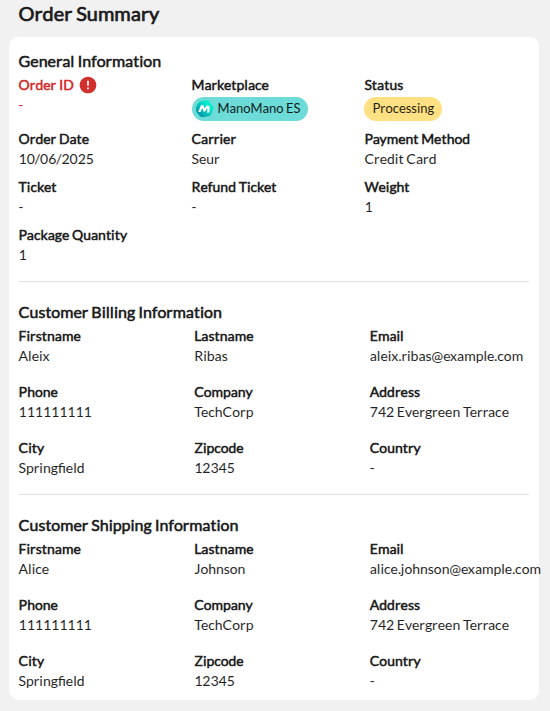
\includegraphics[width=\linewidth]{figures/design_develop/screenshots/tarjeta_resumen_despues_guardar.png}
        \caption{Tarjeta de resumen del pedido después de intentar guardar, mostrando un error.}
    \end{subfigure}
    \par\vspace{0.3cm}
    \caption{Tarjeta de resumen del pedido antes y después de intentar guardar.}
    \label{fig:dev:ss:tarjeta_resumen_pedido}
\end{figure}

\subsubsection{Vista de productos}
\label{dev:subsubsec:vista_productos}

La vista de productos es otra de las vistas principales de la plataforma, ya que permite gestionar todos los productos disponibles en los distintos canales de venta. En este caso, la vista se ha dividido en dos partes:
\begin{itemize}
    \item \textbf{Vista general de productos}: Esta vista permite al usuario ver todos los productos disponibles en la plataforma, independientemente del canal de venta al que pertenezcan. Se pueden filtrar los productos por el canal de venta, además de poder buscarlos por su nombre o \gls{sku}.
    \item \textbf{Vista detallada de producto}: Esta vista permite al usuario ver un producto concreto, así como editarlo. Se pueden ver todos los detalles del producto, incluyendo su nombre, descripción, precio y otros atributos. También se pueden editar los atributos del producto para cada uno de los canales de venta disponibles, lo que permite personalizar el producto según las necesidades de cada canal.
\end{itemize}

\begin{figure}[H]
    \centering
    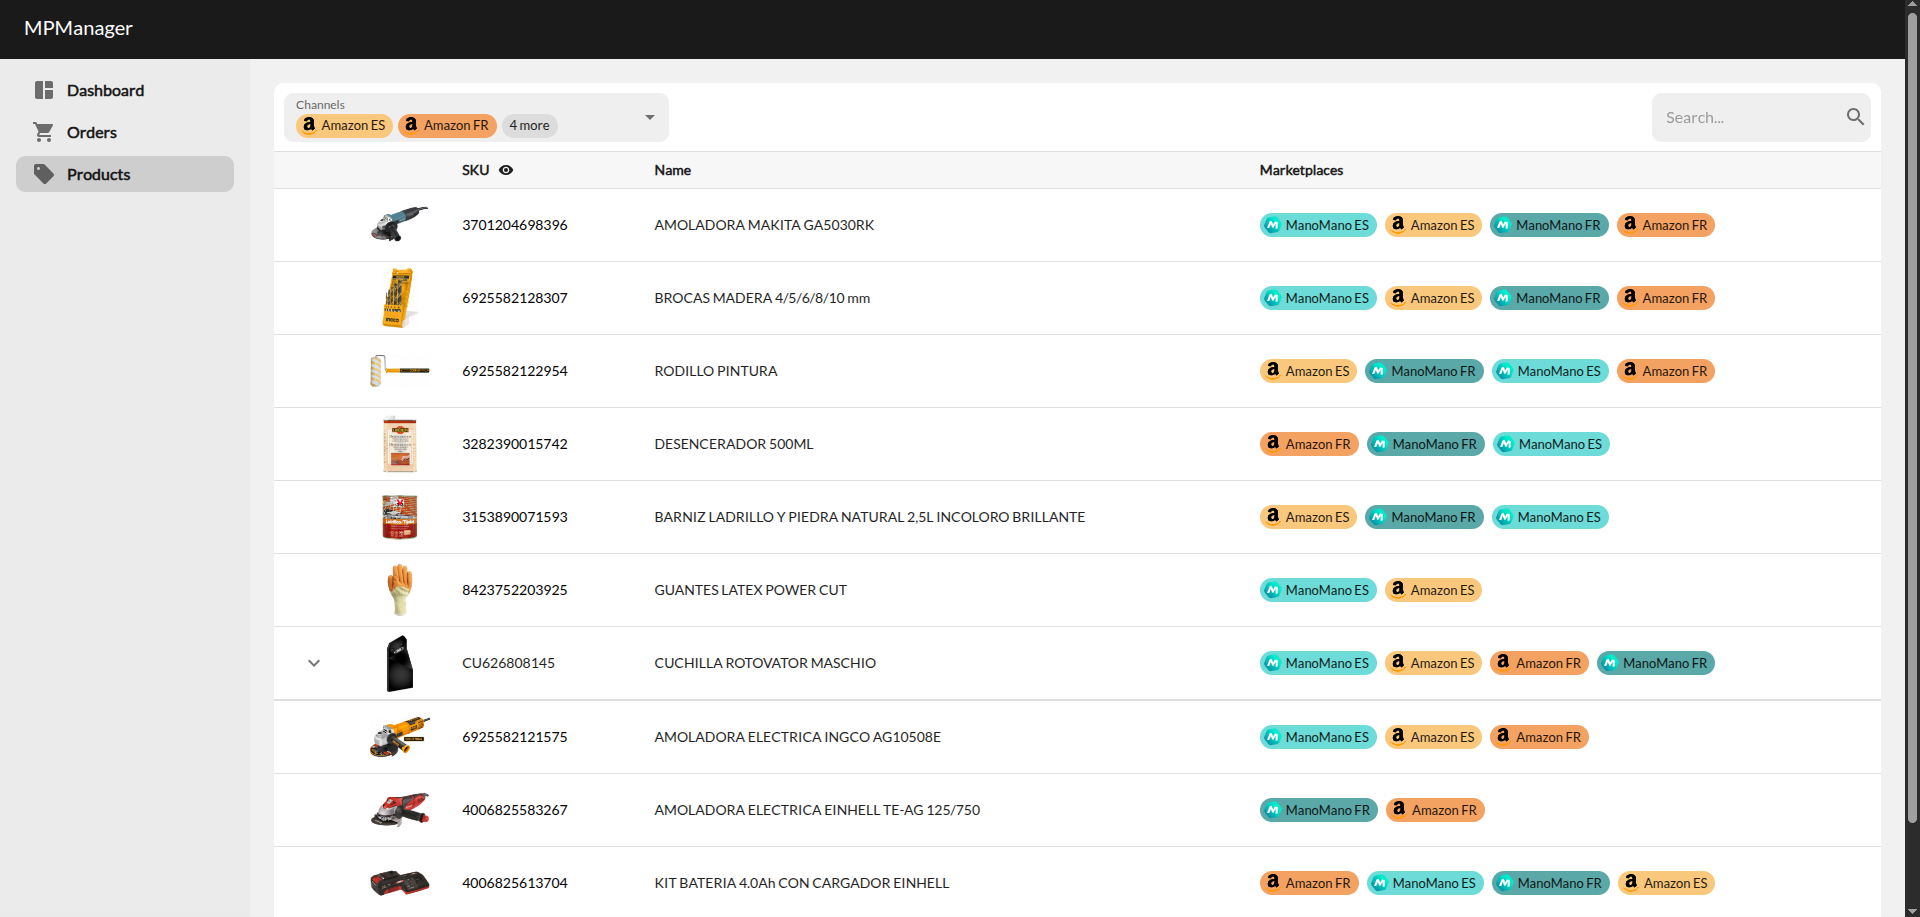
\includegraphics[width=0.8\textwidth]{figures/design_develop/screenshots/tabla_productos.png}
    \caption{Vista general de productos con algunos productos de ejemplo.}
    \label{fig:dev:ss:vista_general_productos}
\end{figure}

Empezando con la vista general de productos, esta es la que se muestra en la figura \ref{fig:dev:ss:vista_general_productos}. Esta vista está basada en la vista general de pedidos, ya que está compuesta por una única tabla que muestra los productos disponibles en la plataforma. En esta tabla se muestra el \gls{sku} del producto, el nombre y los \textit{marketplaces} en los que está disponible. Cuenta también con un campo de búsqueda que permite filtrar los productos por su nombre o \gls{sku}, y un filtro por canal de venta que permite ver únicamente los productos de los canales seleccionados.

Al igual que en la vista de pedidos, la tabla cuenta con paginación, de manera que por defecto se muestran 10 productos. No obstante, el usuario puede cambiar el número de productos por página a 25, 50 o 100. El funcionamiento es exactamente el mismo que en la vista de pedidos, es decir, cada vez que se cambia de página, se realiza una petición al \textit{backend} para obtener los productos correspondientes a la página, búsqueda o filtros seleccionados.

El filtro de canal de venta tiene una particularidad: permite filtrar productos que no están asignados a ningún canal de venta. Esto es útil para identificar productos que aún no se han asignado a ningún canal y que, por lo tanto, no están disponibles para la venta. Para ello, se ha añadido una opción en el filtro que permite seleccionar ``\textit{None}'', lo cual mostrará únicamente los productos que no están asignados a ningún canal.

Por otro lado, para manejar las variantes de un producto, se ha implementado un sistema de agrupación. Esto significa que, si un producto tiene variantes (por ejemplo, diferentes tallas o colores), todas las variantes se agrupan bajo la misma fila de la tabla. Desplegando la fila, se pueden ver todas las variantes del producto y sus respectivos canales de venta. Este comportamiento se puede observar en la figura \ref{fig:dev:ss:variantes_productos}, donde se muestra un producto con dos variantes agrupadas. Remarcar que los canales que se muestran en el producto padre son los canales en los que están sus variantes, y no los canales en los que está el producto padre; el producto padre es una abstracción que se utiliza para agrupar las variantes de un producto y no tiene un canal de venta asociado.

\begin{figure}[H]
    \centering
    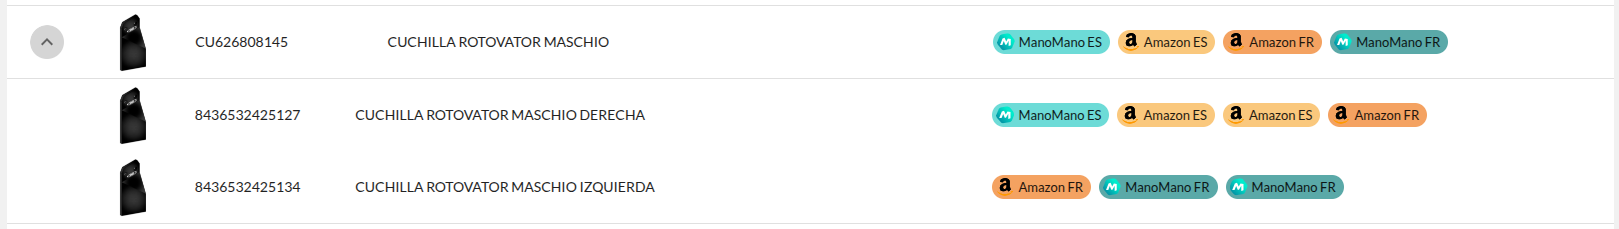
\includegraphics[width=0.8\textwidth]{figures/design_develop/screenshots/variantes_producto.png}
    \caption{Agrupación de variantes de un producto en la vista general de productos.}
    \label{fig:dev:ss:variantes_productos}
\end{figure}

Finalmente, para cargar la vista se realizan dos peticiones al \textit{backend}: una para obtener los productos y otra para obtener los canales de venta disponibles. Todos los componentes que componen la vista se encuentran en la carpeta \texttt{src/components/products/products-list} y son llamados desde el archivo \texttt{src/routes/products/index.tsx}, que es el encargado de definir la ruta.

\begin{figure}[H]
    \centering
    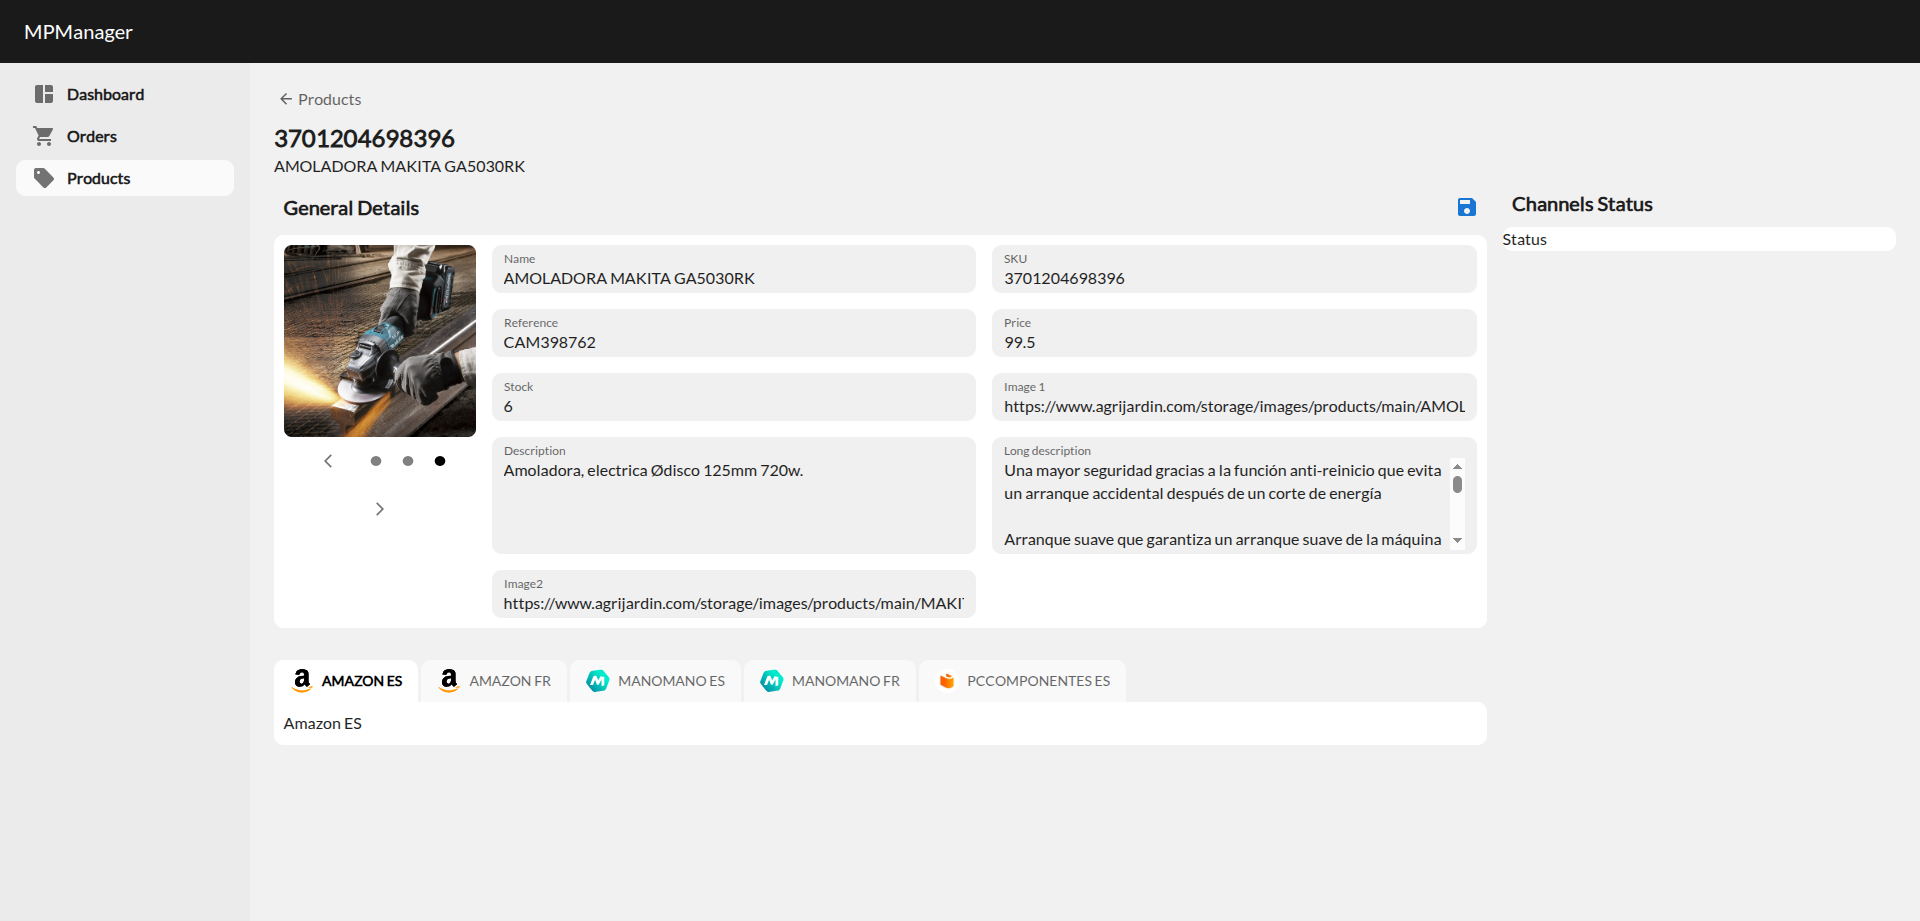
\includegraphics[width=0.8\textwidth]{figures/design_develop/screenshots/detalle_producto.png}
    \caption{Vista detallada de un producto concreto.}
    \label{fig:dev:ss:vista_detallada_productos}
\end{figure}

Pulsando sobre un producto concreto de la tabla, se accede a su vista detallada, que se muestra en la figura \ref{fig:dev:ss:vista_detallada_productos}. En esta vista se pueden ver dos secciones principales: la información general del producto y la información del producto en cada canal de venta.

La primera sección muestra la información general del producto, incluyendo sus atributos genéricos, como el nombre, el \gls{sku} y el precio, y sus atributos asignables, como las descripciones, las imágenes, entre otros. Este componente está preparado para que, si se crean nuevos tipos de atributo desde el \textit{backend}, se añadan automáticamente sus campos correspondientes.

Como característica destacable de esta primera sección, se incluye un carrusel de imágenes que permite al usuario visualizar todas las imágenes asociadas al producto. Este carrusel funciona detectando automáticamente todos los atributos cuyo \textit{key} sea \texttt{image} y mostrando su valor correspondiente, es decir, cada una de las imágenes del producto.

Por otro lado, la segunda sección muestra la información del producto en cada canal de venta. El componente tiene tantas pestañas como canales de venta existan, de manera que el usuario puede navegar entre ellas para ver la información del producto en cada canal. En cada pestaña se muestran los atributos del producto en ese canal, permitiendo al usuario editar los valores de los atributos específicos de cada canal. Esto es útil para personalizar el producto según las necesidades de cada \textit{marketplace}, pues cada uno de ellos puede tener diferentes requisitos o características. Además, desde cada pestaña se puede habilitar o deshabilitar el producto en ese canal de venta, lo que permite al usuario controlar la disponibilidad del producto dependiendo del \textit{marketplace}.

Para guardar los cambios realizados, tanto de atributos de producto como de atributos de producto de canal de venta, el usuario debe pulsar el icono de guardado que se encuentra en la parte superior derecha de cada sección. Esto enviará una petición al \textit{backend} con los nuevos valores de los atributos del producto.

Por último, para cargar la vista detallada de un producto se realizan dos peticiones al \textit{backend}: una para obtener el producto, con todos sus atributos, y otra para obtener los canales de venta disponibles. Todos los componentes que componen la vista se encuentran en la carpeta \texttt{src/components/products/products-detail} y son llamados desde el archivo \texttt{src/routes/products/\$productId.tsx}, que es el encargado de definir la ruta.

\subsubsection{Vista de inicio}
\label{dev:subsubsec:vista_inicio}
La vista de inicio es la última de las vistas principales de la plataforma y proporciona una visión general del estado de los pedidos y productos. Es la primera pantalla que el usuario encuentra al acceder a la aplicación, y está pensada para ofrecer información relevante de forma rápida, sin necesidad de navegar por las distintas secciones.

\begin{figure}[H]
    \centering
    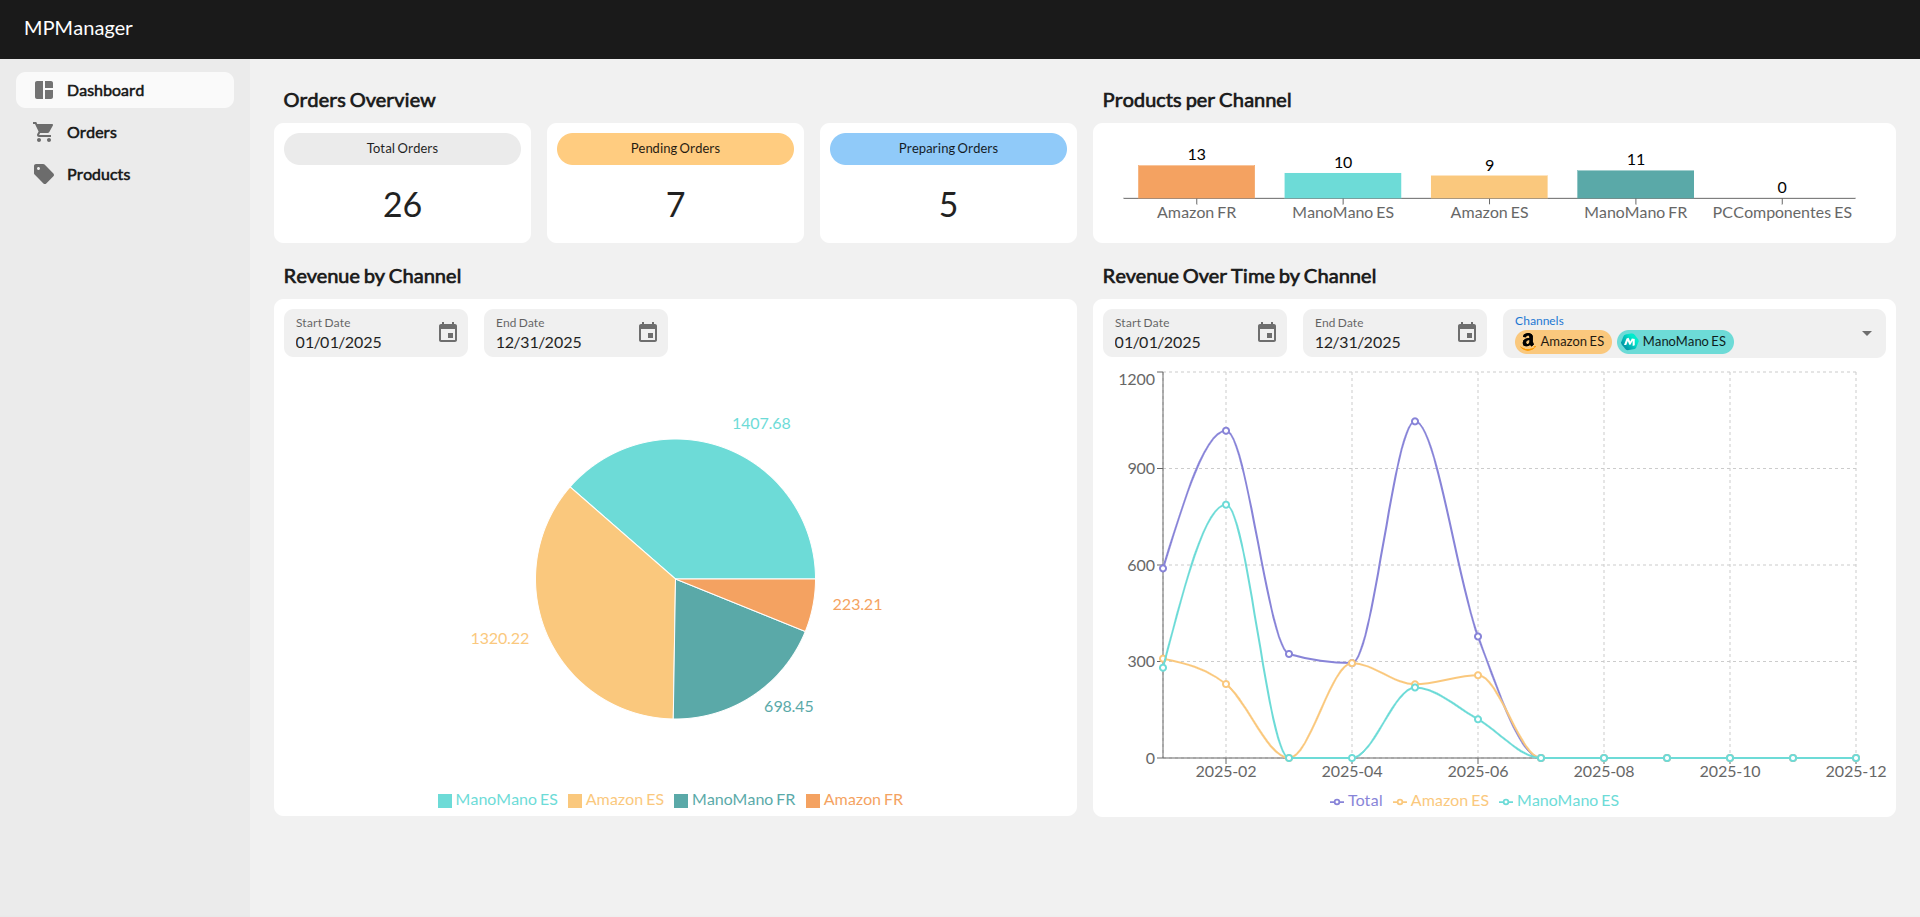
\includegraphics[width=0.8\textwidth]{figures/design_develop/screenshots/dashboard.png}
    \caption{Vista de inicio de la plataforma.}
    \label{fig:dev:ss:vista_inicio}
\end{figure}

El \textit{dashboard} ha sido diseñado para mostrar de un vistazo el rendimiento de los distintos canales de venta. Para transmitir esta información de forma clara y visual, se ha optado por el uso de gráficos, lo cual ha requerido una evaluación previa de distintas librerías. En este análisis se han tenido en cuenta factores como la facilidad de uso, la escalabilidad y la capacidad de personalización. Finalmente, se ha elegido la librería Recharts, que destaca por su integración con React y TypeScript, su flexibilidad y su facilidad de implementación. Recharts permite crear gráficos de barras, de líneas, circulares, entre otros, y ofrece una amplia variedad de opciones de personalización para adaptarlos a las necesidades específicas.

Con la librería para implementar gráficos definida, se ha dividido la vista en cuatro secciones principales, que corresponden a cuatro componentes:

\begin{enumerate}
    \item \textbf{Resumen de pedidos:} \\
          Este componente proporciona una visión general del estado de los pedidos en la plataforma, permitiendo al usuario saber rápidamente si tiene trabajo de preparación pendiente. Para ello, se presentan tres bloques informativos: el número total de pedidos, el número de pedidos pendientes y el número de pedidos en preparación.
    \item \textbf{Productos por canal:} \\
          Este componente muestra un gráfico de barras que representa el número de productos disponibles en cada canal de venta. Esto permite al usuario ver rápidamente en qué canales tiene más productos y dónde podría necesitar añadir más.
    \item \textbf{Ingresos por canal:} \\
          Este componente muestra un gráfico circular que representa los ingresos generados por cada canal de venta. Esto permite al usuario ver rápidamente qué canales son más rentables y dónde podría necesitar centrar sus esfuerzos. Para permitir un mayor control sobre los datos mostrados, se ha añadido un filtro por fecha que permite al usuario seleccionar el rango de fechas para el que se quieren ver los ingresos. Este filtro es opcional, y si no se selecciona, se mostrarán los ingresos del año actual.
    \item \textbf{Ingresos por canal a lo largo del tiempo:} \\
          Este componente muestra un gráfico de líneas que representa los ingresos generados por cada canal de venta o en total a lo largo del tiempo. Esto permite al usuario ver la evolución de los ingresos y detectar tendencias o patrones en el comportamiento de los canales de venta. Al igual que en el componente anterior, se ha añadido un filtro por fecha que permite al usuario seleccionar el rango de fechas para el que se quieren ver los ingresos. También se ha añadido un filtro por canal de venta que permite al usuario seleccionar qué canales de venta quiere ver en el gráfico. Por defecto, se muestra el rango de fechas correspondiente al año actual y el total de ingresos de todos los canales de venta.
\end{enumerate}

Para cargar la vista de inicio se realizan cinco peticiones al \textit{backend}: una petición para cada uno de los cuatro componentes y una petición para obtener los canales de venta disponibles. Además, por cada actualización de los filtros de fecha o canal de venta, se realiza una nueva petición al \textit{backend} para obtener los datos actualizados. Por otro lado, todos los componentes que forman la vista se encuentran en la carpeta \texttt{src/components/dashboard} y son llamados desde el archivo \texttt{src/routes/index.tsx}, que es el encargado de definir la ruta.

\begin{figure}[H]
    \centering
    \begin{subfigure}{0.48\linewidth}
        \centering
        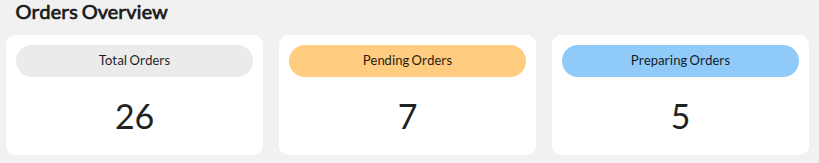
\includegraphics[width=\linewidth]{figures/design_develop/screenshots/dash_sec1.png}
        \caption{Sección de resumen de pedidos.}
    \end{subfigure}
    \hfill
    \begin{subfigure}{0.48\linewidth}
        \centering
        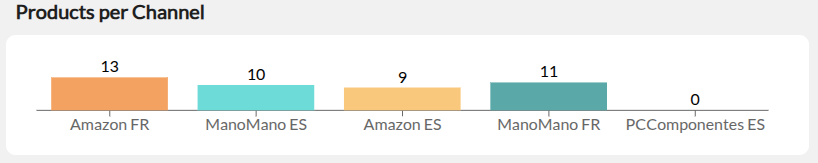
\includegraphics[width=\linewidth]{figures/design_develop/screenshots/dash_sec2.png}
        \caption{Sección de productos por canal.}
    \end{subfigure}
    \par\vspace{0.6cm}
    \begin{subfigure}{0.48\linewidth}
        \centering
        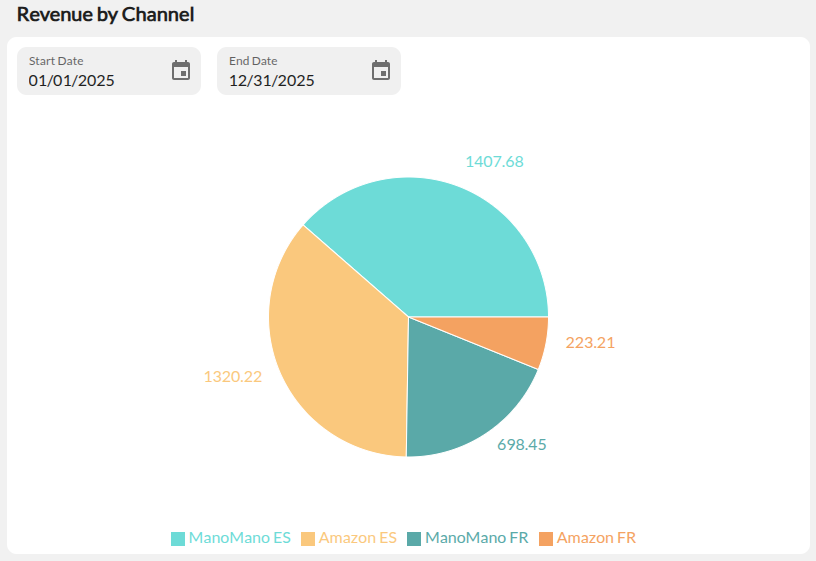
\includegraphics[width=\linewidth]{figures/design_develop/screenshots/dash_sec3.png}
        \caption{Sección de ingresos por canal filtrado por el último año.}
    \end{subfigure}
    \hfill
    \begin{subfigure}{0.48\linewidth}
        \centering
        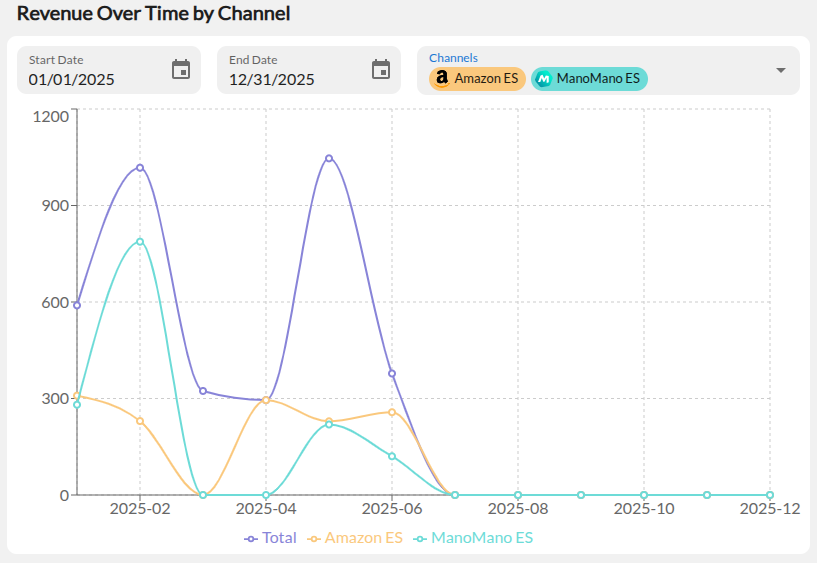
\includegraphics[width=\linewidth]{figures/design_develop/screenshots/dash_sec4.png}
        \caption{Sección de ingresos por canal a lo largo del tiempo filtrado por el último año.}
    \end{subfigure}
    \par\vspace{0.3cm}
    \caption{Secciones de la vista de inicio.}
    \label{fig:dev:ss:vista_inicio_secciones}
\end{figure}

Todo este conjunto de gráficos y datos representa una primera iteración de lo que en un futuro se pretende que sea un panel de control más completo y detallado. La idea es que, a medida que la plataforma evolucione, se puedan añadir más gráficos y datos relevantes para el usuario, de manera que este tenga acceso a un conjunto de herramientas que le permitan analizar como están funcionando los distintos canales de venta y tomar decisiones informadas.